\documentclass[12pt, a4paper, final, twoside]{report}

\newcommand{\isPrintVersion}{false}						% false -> show colored links, true -> all links in black

\usepackage[utf8]{inputenc}
\usepackage[T1]{fontenc}
\usepackage{textcomp}
\usepackage{url}
%%%%%%%%%%%%%%%%%%%%%%%%%%%%%%%%%%%%%%%%%%%%%%%%%%%%%%%%%%%%%%%%%%%%%%%%%%%%%%%%
%%%%%%%%%%%%%%%%%%%%%%%%%%%%%%% Data  %%%%%%%%%%%%%%%%%%%%%%%%%%%%%%%%%%%%%%%%%%
\newcommand{\thesisTitle}{Tic Tac Toe}
\newcommand{\authorName}{Barkouki Oussama et Hayaoui Abdelhakim}

\newcommand{\signatureDate}{29 Janvier 2020}
\newcommand{\city}{Rabat}

%%%%% Title page
\newcommand{\reportType}{Rapport Projet C}
\newcommand{\university}{École nationale supérieure d'informatique et d'analyse des systèmes}


\newcommand{\course}{2019/2020}
\newcommand{\supervisorName}{Mr. M. EL HAMLAOUI}


\newcommand{\byTitle}{par}
\newcommand{\courseOfStudiesTitle}{Année universitaire}
\newcommand{\courseTitle}{Course}
\newcommand{\supervisorTitle}{Professeur encadrant : }

\newcommand{\universityLogo}{ensias.PNG}
\newcommand{\companyLogo}{UMF5.PNG}

%%%%% Quote

%%%%% Declaration
\newcommand{\declaration}{C’est parce que nous avons beaucoup estimé tous ceux qui nous ont écoutés, conseillés, critiqués et encadrés que nous tenons à leur faire part de toutes nos gratitudes, et plus particulièrement, nous tenons à remercier à travers ces courtes lignes : \\
Monsieur Mahmoud EL HAMLAOUI professeur à l’ENSIAS, qui a accepté d’examiner et d’encadrer ce travail pour le valoriser malgré ses nombreuses occupations.  Nos remerciements vont également à nos professeurs des modules de « Structures de données » : Monsieur Abdellatif EL FAKER pour son entière disponibilité, « Algorithmique » : Monsieur Ahmed ETTALBI pour le savoir qu’il nous a transmis et de « Techniques de programmation » : Monsieur Hatim Guermah.  Enfin, nos remerciements s’adressent aux professeurs et au corps administratif de l’Ecole Nationale Supérieure de l’Informatique et de l’Analyse des Systèmes.
}

\newcommand{\declarationTitle}{Remerciements}
\newcommand{\ListOfFiguresTitle}{List of Figures}
\newcommand{\ListOfTablesTitle}{List of Tables}

%%%%% Document
\title{\thesisTitle}
\author{\authorName}

%%%%%%%%%%%%%%%%%%%%%%%%%%%%%%%%%%%%%%%%%%%%%%%%%%%%%%%%%%%%%%%%%%%%%%%%%%%%%%%%
%%%%%%%%%%%%%%%%%%%%%%%%%%%%%%%% Abstract  %%%%%%%%%%%%%%%%%%%%%%%%%%%%%%%%%%%%%
\usepackage{abstract}
\renewcommand{\abstractnamefont}{\large\bfseries}

\newcommand{\abstractText}{Tic-tac-toe is a paper-and-pencil game for two players, X and O, who take turns marking the spaces in a 3×3 grid. The player who succeeds in placing three of their marks in a horizontal, vertical, or diagonal row is the winner.

This document is a summary of our programming project. This project aims to create the game of Tic-tac-toe in C language.

To do so, we started, first of all by understanding the game and the objectives to be achieved. Then studies of the specifications that will be conducted to extract the different tasks requested and deduce the features that will be implemented in the game.

Then we tried to get a clear idea about the design by creating a wireframe which allowed us to get also a visual guide that represents the skeletal framework of the project.

Finally, we focused on the game development phase. As part of this phase, we started with the administration, authentication and data backup functions, and then moved on to the implementation of the play algorithms, and then we ran some test to ensure the proper functioning of the game.

}



%%%%%%%%%%%%%%%%%%%%%%%%%%%%%%%%%%%%%%%%%%%%%%%%%%%%%%%%%%%%%%%%%%%%%%%%%%%%%%%%
%%%%%%%%%%%%%%%%%%%%%%%%%%%%%%%% Packages  %%%%%%%%%%%%%%%%%%%%%%%%%%%%%%%%%%%%%
\usepackage[left=3.5cm,right=2.5cm,top=3cm,bottom=2.5cm]{geometry}
\usepackage[ngerman,english]{babel}
\usepackage{amsmath}
\usepackage{amsfonts}
\usepackage{amssymb}
\usepackage{enumitem}
\usepackage{float}
\usepackage{fancyhdr}
\usepackage[bottom]{footmisc}
\usepackage[printonlyused]{acronym}
\usepackage{appendix}
\usepackage{pdfpages}
\usepackage{ifthen}
\usepackage{csquotes}
\usepackage{emptypage}

%%%%%%%%%%%%%%%%%%%%%%%%%%%%%%%%%%%%%%%%%%%%%%%%%%%%%%%%%%%%%%%%%%%%%%%%%%%%%%%%
%%%%%%%%%%%%%%%%%%%%%%%%%%%%%% Colors  %%%%%%%%%%%%%%%%%%%%%%%%%%%%%%%%%%%%%%%%%
\definecolor{darkBlue}{cmyk}{0.9592, 0.4592, 0, 0.6157} % {HTML}{043562}
\definecolor{lightBlue}{cmyk}{0.5, 0.25, 0, 0.2} 		% {HTML}{6699cc}
\definecolor{darkGrey}{cmyk}{0, 0, 0, 0.9333} 			% {HTML}{111111}
\definecolor{lightGrey}{cmyk}{0.0164, 0.0082, 0, 0.0431}% {HTML}{F0F2F4}
\definecolor{magenta}{cmyk}{0, 1, 0.4972, 0.3059}		% {HTML}{B10059}

%%%%%%%%%%%%%%%%%%%%%%%%%%%%%%%%%%%%%%%%%%%%%%%%%%%%%%%%%%%%%%%%%%%%%%%%%%%%%%%%
%%%%%%%%%%%%%%%%%%%%%%%%%%%%%% New commands  %%%%%%%%%%%%%%%%%%%%%%%%%%%%%%%%%%% 

%%%%% Caption with sources
\usepackage{caption}
\captionsetup{justification=centering}
\newcommand{\captionsource}[2][]{
	\ifthenelse{\equal{#1}{}}
		{\small\textit{Source: #2}} % if empty
		{\small\textit{Source: #2, \href{#1}{#1}} % else
	}
}

%%%%% Theorems / Definitions
\usepackage{amsthm} 					
\newtheorem{define}{Definition}

%%%%% Code in text
\newcommand{\code}[1]{{\ttfamily#1}}

%%%%%%%%%%%%%%%%%%%%%%%%%%%%%%%%%%%%%%%%%%%%%%%%%%%%%%%%%%%%%%%%%%%%%%%%%%%%%%%%
%%%%%%%%%%%%%%%%%%%%%%%%%%%%%% Bibliography  %%%%%%%%%%%%%%%%%%%%%%%%%%%%%%%%%%%
\usepackage[backend=bibtex,style=numeric,citestyle=numeric]{biblatex}
\bibliography{bibliography} 

% linebreaks in bibliography urls
\usepackage{url}
\usepackage{breakurl}
\def\UrlBreaks{\do\/\do-}							% add a breakpoint at - and /

\setcounter{biburlnumpenalty}{1000}  				% add a breakpoint after all numbers
\setcounter{biburlucpenalty}{1000}					% add a breakpoint after all uppercase letters
\setcounter{biburllcpenalty}{1000}   				% add a breakpoint after all lowercase letters

%%%%%%%%%%%%%%%%%%%%%%%%%%%%%%%%%%%%%%%%%%%%%%%%%%%%%%%%%%%%%%%%%%%%%%%%%%%%%%%%
%%%%%%%%%%%%%%%%%%%%%%%%%%%%%%% PDF settings  %%%%%%%%%%%%%%%%%%%%%%%%%%%%%%%%%%
\usepackage[pdftitle={\thesisTitle}, pdfauthor={\authorName},pdfsubject={\thesisTitle}, pdfcreator={pdflatex}, pdfpagemode=UseOutlines, pdfdisplaydoctitle=true, pdflang={en}, breaklinks]{hyperref}

% color settings for links in pdf
\ifthenelse{\equal{\isPrintVersion}{true}}
{ % print version
	\hypersetup{
		hidelinks=true,
		colorlinks=false, 
		linktocpage=true, 							% page numbers are clickable
		bookmarksnumbered=true 						% show heading numbering in pdf table of contents
	}
}{ % screen version
	\hypersetup{
		colorlinks=true, 
		linkcolor=darkBlue,
		citecolor=darkBlue,
		filecolor=darkBlue,
		menucolor=darkBlue,
		urlcolor=darkBlue,
		linktocpage=true, 							% page numbers are clickable
		bookmarksnumbered=true 						% show heading numbering in pdf table of contents
	}
}

%%%%%%%%%%%%%%%%%%%%%%%%%%%%%%%%%%%%%%%%%%%%%%%%%%%%%%%%%%%%%%%%%%%%%%%%%%%%%%%%
%%%%%%%%%%%%%%%%%%%%%%%%%%%%%%% Typography  %%%%%%%%%%%%%%%%%%%%%%%%%%%%%%%%%%%%
\usepackage{lmodern}
\usepackage{mathpazo}
\fontfamily{ppl}\selectfont

\setlength{\parskip}{8pt}							% after paragraph
\setlength{\parindent}{0pt}							% new paragraph indent
\renewcommand{\baselinestretch}{1.2}\normalsize		% line height (line height for content is defined in line 281)

% Prevent widows and orphans
\clubpenalty = 10000								% prevent orphans
\widowpenalty = 10000 								% prevent widows
\displaywidowpenalty=10000

% Headings
\usepackage{titlesec}
\newcommand{\hsp}{\hspace{20pt}}

\titleformat{\chapter}[block]{\Huge\bfseries}{\thechapter \hsp {|}\hsp}{0pt}{\Huge\bfseries}
\titleformat{\section}[block]{\Large\bfseries}{\thesection \ }{0pt}{\Large \bfseries}
\titleformat{\subsection}[block]{\large\bfseries}{\thesubsection \ }{0pt}{\large \bfseries}
%%%%%%%%%%%%%%%%%%%%%%%%%%%%%%%%%%%%%%%%%%%%%%%%%%%%%%%%%%%%%%%%%%%%%%%%%%%%%%%%
%%%%%%%%%%%%%%%%%%%%%%%%%%%%%%%%%%% Listings  %%%%%%%%%%%%%%%%%%%%%%%%%%%%%%%%%%
\usepackage{listings}

\lstset{
	language=Java,								% default language
	numbers=left,								% line number position, alternative: none
	stepnumber=1,								 
	numbersep=6pt,								% distance between line number and code
	numberstyle=\fontsize{9pt}{9pt}\ttfamily,	% line number style
	breaklines=true,							% break lines if necessary
	breakautoindent=true,						% indent after line break
	postbreak=\space,							% break at space
	tabsize=4,									% tab size
	showspaces=false,							% do not show spaces in code
	showstringspaces=false,						% do not show spaces in strings
	extendedchars=true,							% use Latin1
	captionpos=b,								% caption position
	backgroundcolor=\color{lightGrey}, 			% background color
	xleftmargin=0pt,								
	xrightmargin=0pt,							
	frame=leftline,								% draw frame ar left side only
	framerule=1.1pt,							% frame width
	frameround=ffff,							% round corners: f = not rounded | t = rounded
	rulecolor=\color{lightBlue},				% frame color
	framesep=1.5pt,								% distance between line number and border 
	fillcolor=\color{lightGrey},
	basicstyle=\ttfamily\footnotesize\color{darkGrey},	
	keywordstyle=\color{magenta}\bfseries,
	identifierstyle=,
	commentstyle=\color{lightBlue},
	stringstyle=\color{darkBlue}
}

\lstloadlanguages{bash, C, C++, HTML, Java, PHP, Python, SQL}

% change heading above listings to \ListOfListingsTitle
\renewcommand{\lstlistlistingname}{\ListOfListingsTitle}

% Group list of listings by chapter
\let\Chapter\chapter
\def\chapter{\addtocontents{lol}{\protect\addvspace{10pt}}\Chapter}

%%%%%%%%%%%%%%%%%%%%%%%%%%%%%%%%%%%%%%%%%%%%%%%%%%%%%%%%%%%%%%%%%%%%%%%%%%%%%%%%
%%%%%%%%%%%%%%%%%%%%%%%%%%%%%%%%%%% Diagrams  %%%%%%%%%%%%%%%%%%%%%%%%%%%%%%%%%%
\usepackage{tikz}
\usetikzlibrary{shapes,arrows,shadows}
% flow diagrams
\tikzstyle{startstop} = [rectangle, rounded corners, minimum width=3cm, minimum height=0.9cm,text centered, draw=lightBlue, fill=lightGrey]
\tikzstyle{io} = [trapezium, trapezium left angle=70, trapezium right angle=110, minimum width=3cm, minimum height=0.9cm, text centered, draw=lightBlue, fill=lightGrey]
\tikzstyle{process} = [rectangle, minimum width=3cm, minimum height=0.9cm, text centered, text width=3cm, draw=lightBlue, fill=lightGrey]
\tikzstyle{decision} = [diamond, minimum width=3cm, minimum height=0.9cm, text centered, draw=lightBlue, fill=lightGrey]
\tikzstyle{arrow} = [thick,->,>=stealth]
\tikzstyle{comment} = [rectangle, minimum width=1cm, minimum height=0.9cm, text centered, text width=3cm, draw=none, fill=none]
\tikzstyle{subprocess} = [rectangle split, rectangle split horizontal, rectangle split parts=3, minimum height=0.9cm, minimum width=3cm, draw=lightBlue, fill=lightGrey]

% sequence diagrams
\usepackage[underline=false]{pgf-umlsd}

%%%%%%%%%%%%%%%%%%%%%%%%%%%%%%%%%%%%%%%%%%%%%%%%%%%%%%%%%%%%%%%%%%%%%%%%%%%%%%%%
%%%%%%%%%%%%%%%%%%%%%%%%%%%%% Todo Comments  %%%%%%%%%%%%%%%%%%%%%%%%%%%%%%%%%%%
\usepackage[colorinlistoftodos]{todonotes}
\reversemarginpar
\setlength{\marginparwidth}{3cm}

\newcommand{\todoQuestion}[1]{\todo[color=green!40]{#1}}
\newcommand{\todoImportant}[1]{\todo[color=red!60]{#1}}

%%%%%%%%%%%%%%%%%%%%%%%%%%%%%%%%%%%%%%%%%%%%%%%%%%%%%%%%%%%%%%%%%%%%%%%%%%%%%%%%
%%%%%%%%%%%%%%%%%%%%%%%%%%%%%%%%%% Structure  %%%%%%%%%%%%%%%%%%%%%%%%%%%%%%%%%%
\begin{document}
	\setlength{\headheight}{24.7pt}					% minimum height required by Latexmk
	\pagenumbering{Roman}

%%%%% Title page, quote, declaration, abstract 
	\fancypagestyle{plain}{ 						% no header, no footer
		\fancyhf{} 
		\fancyfoot{}
		\renewcommand{\headrulewidth}{0pt}
		\renewcommand{\footrulewidth}{0pt}
	}	
	\begin{titlepage}
	\includegraphics[width=4cm]{\companyLogo}
	\hfill
	\includegraphics[width=4cm]{\universityLogo}
	\centering
	
	{\large \ \par}
	{\scshape\LARGE \reportType \par}	
	\vspace{1.5cm}
	{\huge\bfseries \thesisTitle \par}
	\vspace{1.5cm}
	\vspace{1cm}
	{\large \byTitle \par}
	{\Large\itshape \authorName \par}
	\vfill
	\begin{tabbing}
		mmmmmmmmmmmmmmmmmmmmmmmmmm			\= \kill 			% define width

		\textbf{\supervisorTitle}			\> \supervisorName \\
	\end{tabbing}
\end{titlepage}

% ############################################
% ############################################
\cleardoublepage
\chapter*{\declarationTitle}
\declaration
\vspace{4em}

\begin{tabbing}
	mmmmmmmmmmmmmmmmmm	\= \kill 	% define width
	\city, \ \signatureDate 	\> \rule{6cm}{0.4pt} \\
				\> \authorName
\end{tabbing}

% ############################################


% ############################################
\cleardoublepage
\begin{abstract}
	\abstractText
\end{abstract}
\cleardoublepage


%%%%% Table of Contents
	\setlength{\parskip}{0pt}						% after paragraph
	\setcounter{tocdepth}{2}						% depth of table of contents
	\tableofcontents
	\thispagestyle{empty}
		
%%%%% Figures, Tables, Listings	
	\fancypagestyle{plain}{ 
		\fancyhf{} 
		\fancyfoot[LE,RO]{\thepage}
		\renewcommand{\headrulewidth}{0pt}
		\renewcommand{\footrulewidth}{0pt}
	}	
	\addtocounter{page}{6}							% increase page number: +6

	\listoffigures

	%\cleardoublepage



%%%%% Content
	\pagenumbering{arabic}
	\setlength{\parskip}{8pt}						% after paragraph
	\renewcommand{\baselinestretch}{1.4}\normalsize	% line height 
	
	\pagestyle{fancy}
	\fancyhf{}
	\renewcommand{\chaptermark}[1]{\markboth{#1}{}}
	\fancyhead[LE,RO]{\thechapter  \ -- \ \nouppercase\leftmark}
	\fancyfoot[LE,RO]{\thepage}
	% ----------------------------------------------
\chapter{Problématique et cadre général du projet}\label{ch:structure}
La présente partie nous permet de présenter la problématique, identifier toutes les fonctionnalités de notre application, et ceci en recensant les besoins fonctionnels et d’appréhender la liste des exigences traduites par les besoins non fonctionnels, et donner les étapes de la résolution.

% ############################################
\section{Problématique}\label{sec:section1}

Dernièrement, la majorité des enfants spécialement ceux de la génération alpha (nés après 2013)  découvrent la manipulation et les plaisirs de l'ordinateur vers l’âge de  3 ans. Plusieurs familles disposent d'ailleurs des équipements informatiques. Alors que la majorité de ces enfants, utilisent ces équipements dans des jeux ou des plateformes qui influencent négativement leur performances mentales et sociaux. Puisque leurs âge est l’idéal pour l’apprentissage,  c’est préférable d’utiliser l’outil informatique en tous ce qui est éducatif notamment le développent de tout ce qui est logique et stratégie.

Le besoin exprimé se formule comme suit :

\begin{figure}[H]
	\centering
	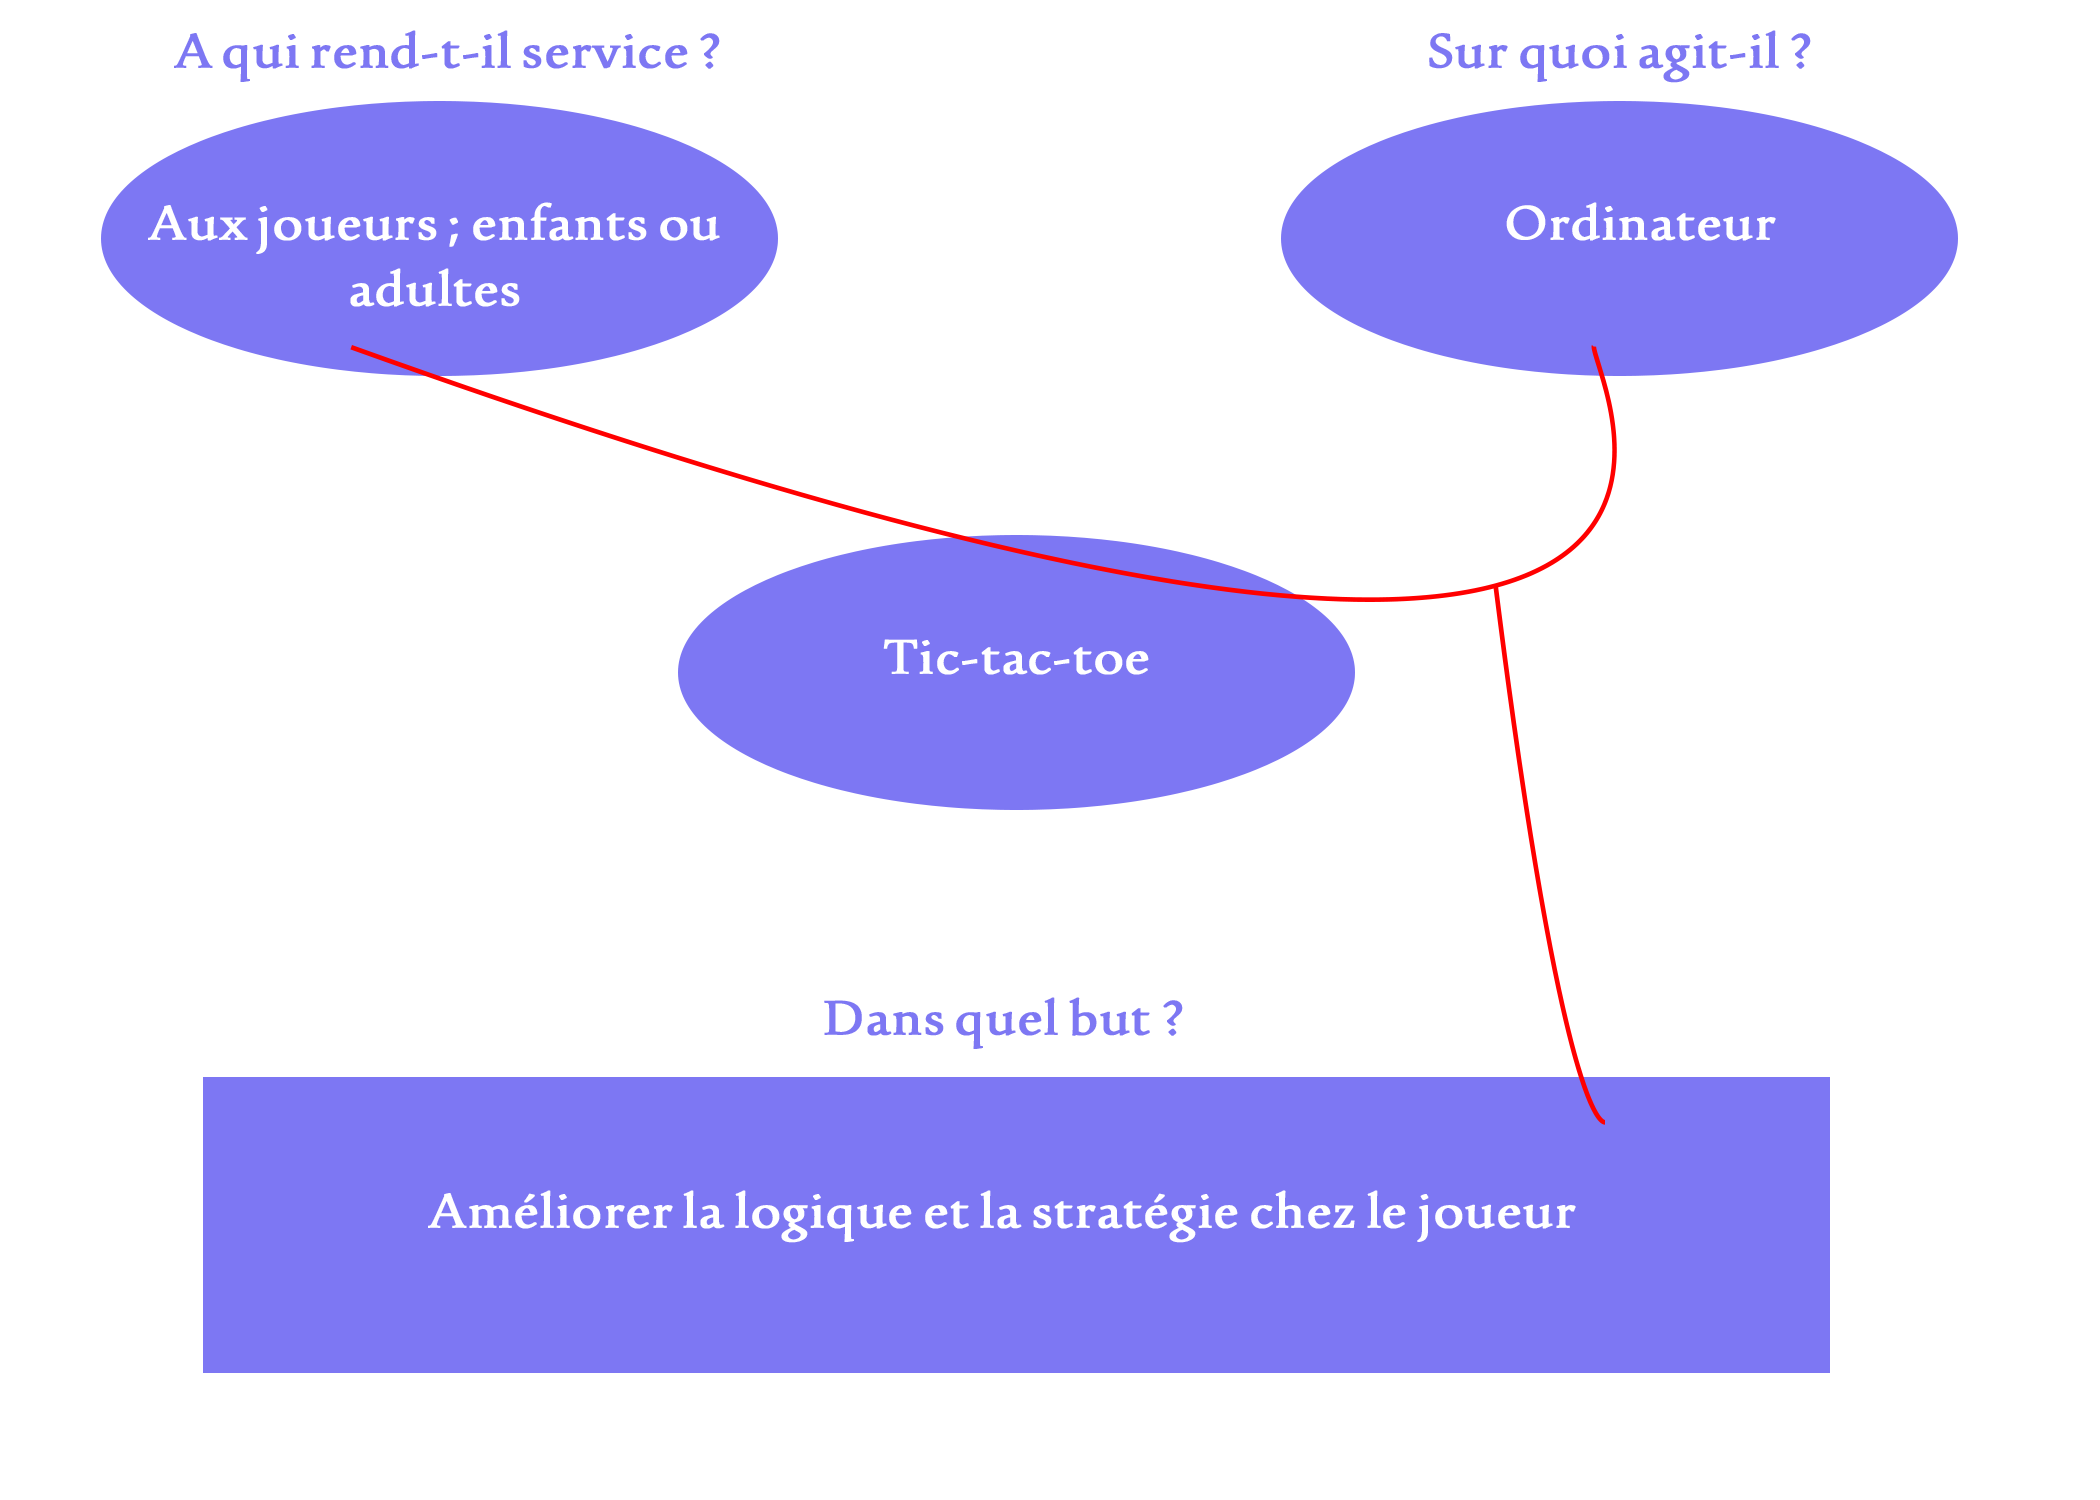
\includegraphics[width=1\textwidth]{bete a corne.PNG}
	  \caption{Diagramme bête à corne du jeu }
	\label{fig: Diagramme bête à corne du jeu }
\end{figure}
\section{Cahier des charges}\label{sec:section2}
\subsection{Contexte et objectifs :}

De nos jour , les gens utilisent les outils informatiques pour jouer même des jeux traditionnels comme tic tac toe, pour cela , on est obligé de finaliser ce jeu qui consiste à assurer une source de défis et de développent de logique.\\
Notre objectif à travers ce travail est de construire ce fameux jeu  qui répond aux besoins de l’utilisateur par la réalisation d’une application nommée « Tic Tac Toe» en développant une application comportant l’ensemble des exigences demandées.

\subsection{Les besoins fonctionnels :}
Après une étude détaillée du système, cette partie est réservée à la description des exigences fonctionnelles des différents acteurs de l’application.
Ces exigences sont :\\
Un joueur peut sans l’existence de l’internet :
\begin{itemize}
\item	 Créer un compte ;
\item	 S’identifier
\item	 Créer une partie et choisir entre jouer contre :
\begin{enumerate}
\item	 Mouvement aléatoires
\item	 Un algorithme (Mini Max Élagage alpha-bêta )
\end{enumerate}


\item	 Voir l’historique des mouvements. 
\item	 Charger une partie déjà enregistrée.
\item	 Voir les dix meilleurs scores.
\item  Consulter la page ‘’ à propos ‘’ 
\end{itemize}

\subsection{Les besoins non fonctionnels :}
Les besoins non fonctionnels décrivent toutes les contraintes techniques, ergonomiques et esthétiques auxquelles est soumis le système pour sa réalisation et pour son bon fonctionnement. Et en ce qui concerne notre application, nous avons dégagé les besoins suivants :
\begin{itemize}
\item  La disponibilité : 
\end{itemize}
 L’application doit être disponible pour être utilisé par n’importe quel utilisateur.
\begin{itemize}
\item  La convivialité de l’interface graphique : 
\end{itemize}
 L’application doit fournir une interface conviviale et simple pour tout type d’utilisateur.
\begin{itemize}
\item  La fiabilité : 
\end{itemize}
Les données fournies par l’application doivent être fiables. La possibilité de retourner au menu principal de l’application à partir de n’importe quelle fenêtre de celle-ci.
\begin{itemize}
\item  La performance  : 
\end{itemize}
Le système doit réagir dans un délai précis, quel que soit l’action de l’utilisateur.
\subsection{Caractéristiques de l’application }
\begin{itemize}
\item  Design simple et conviviale ;
\item Interfaces graphiques ergonomiques ;    
\item  Langue utilisée: anglaise.
\end{itemize}
\section{Les étapes de la résolution du problème}\label{sec:section3}
Pour la résolution du problème on commencer d’abord par une lire bien le cahier de charge et voir une vision sur le concept et le design du jeu, pour cela on a opté à utiliser ce qu’on appelle « frameware » qui est un guide qui représente le cadre squelettique du projet comme on le voit dans la figure suivante :
\clearpage
\begin{figure}[H]
	\centering
	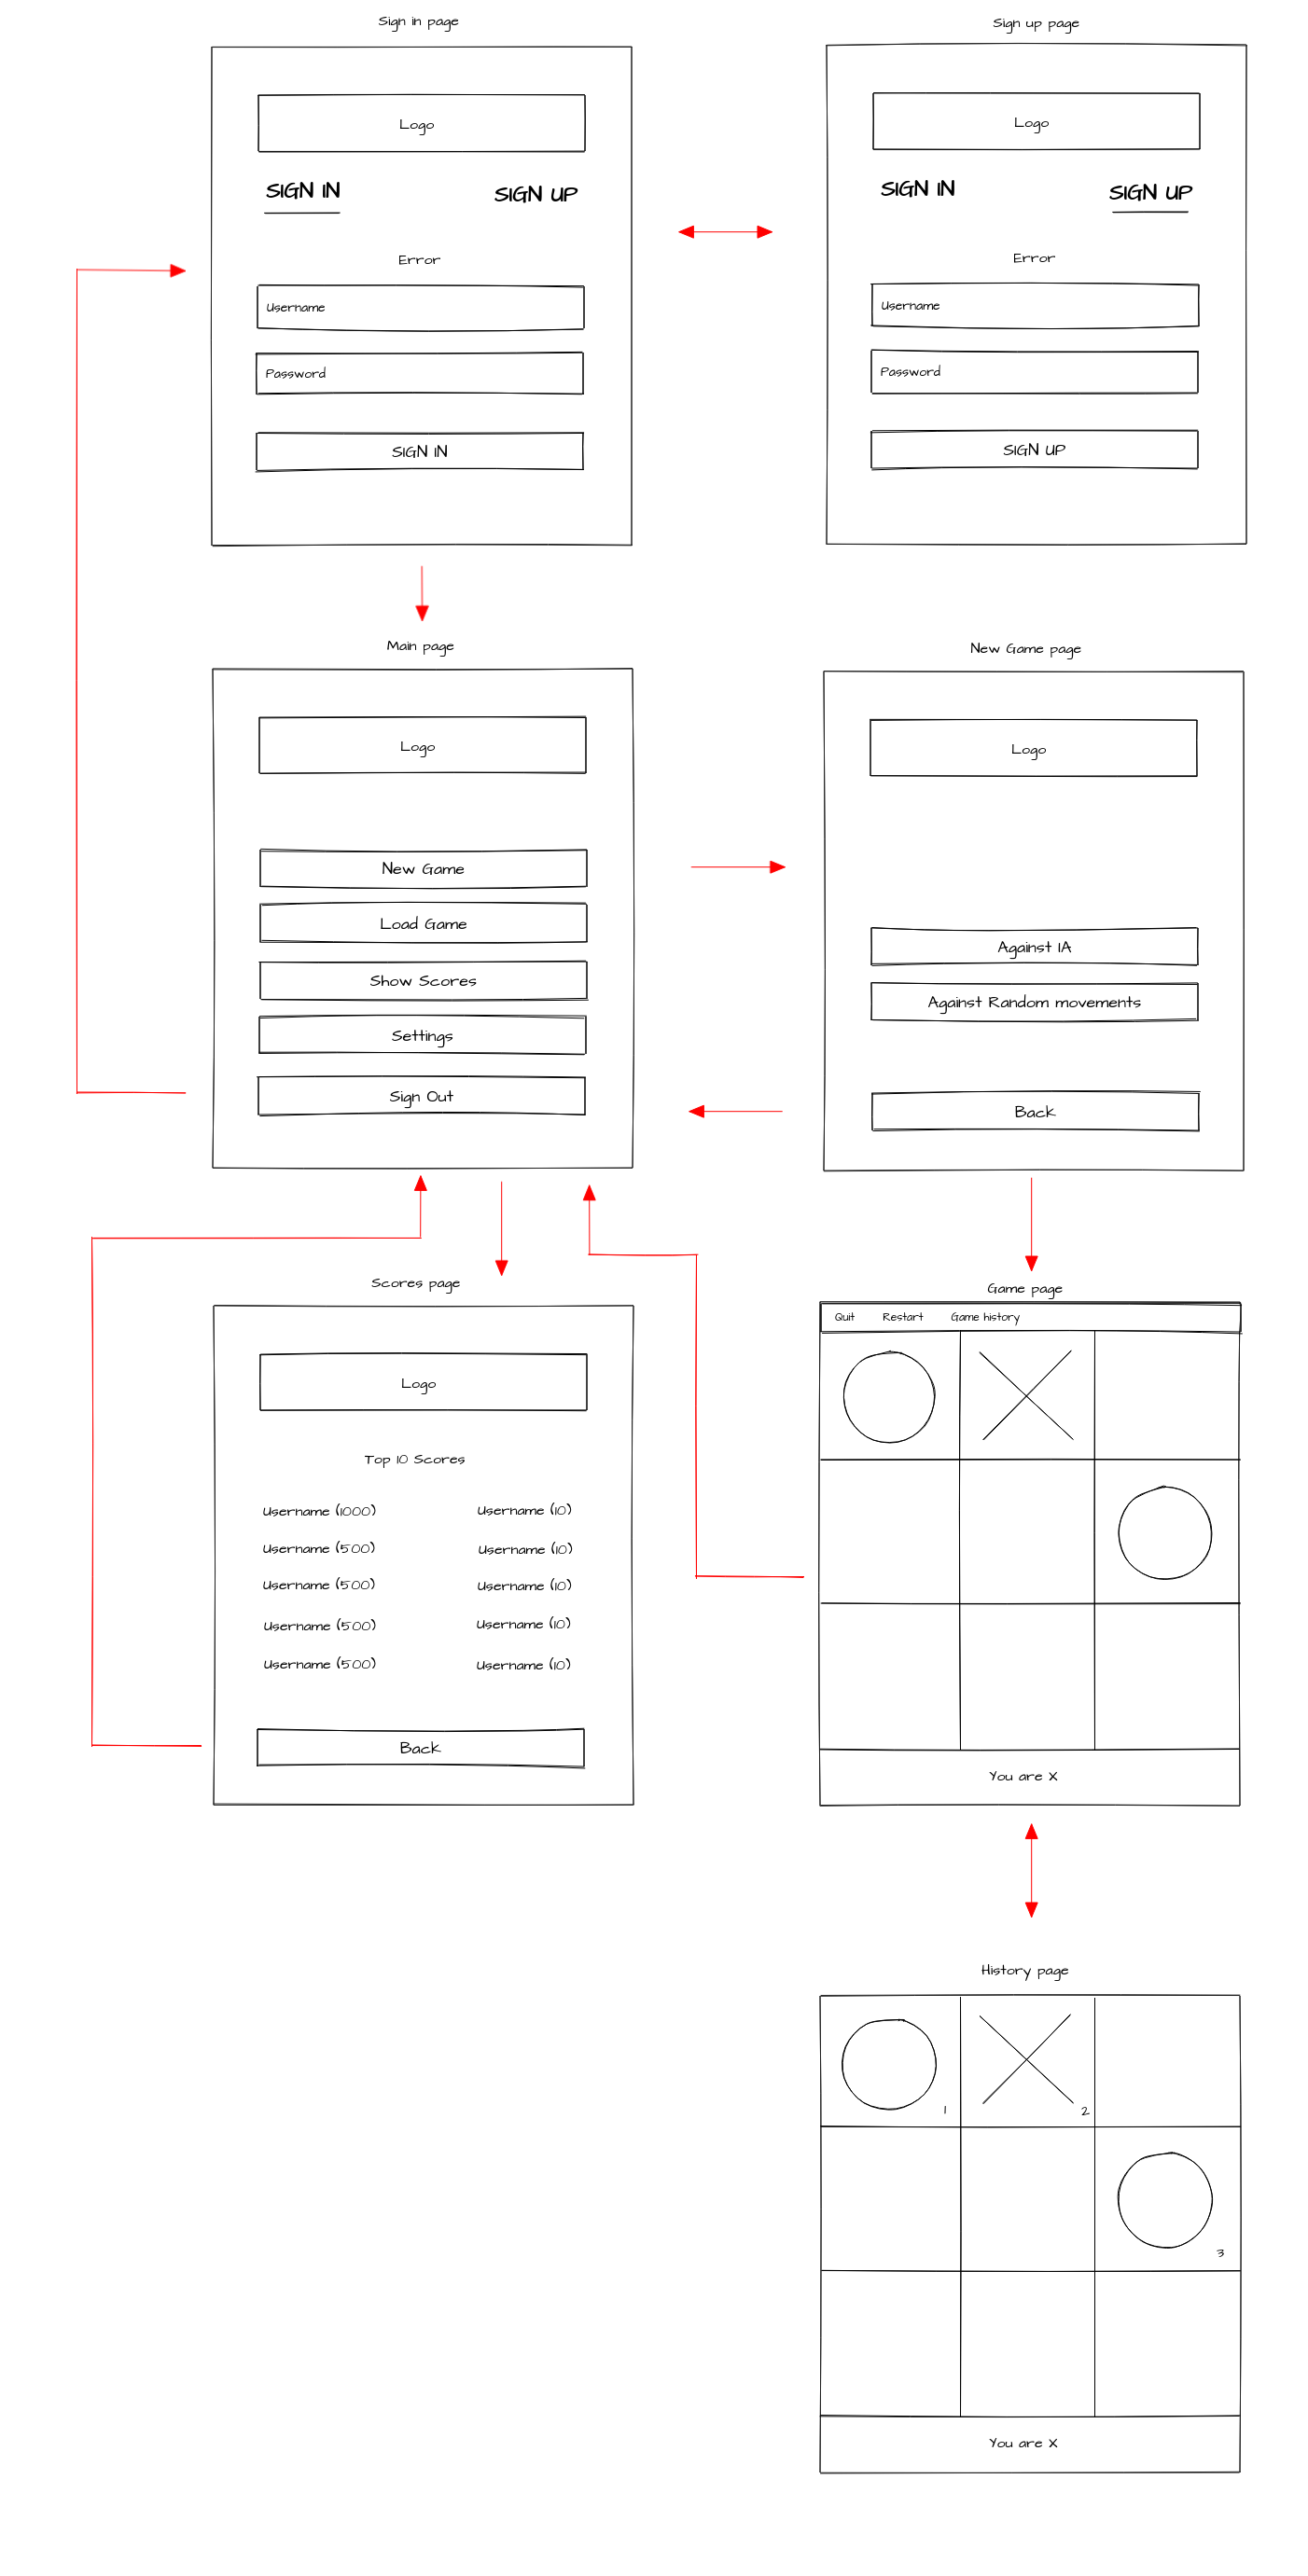
\includegraphics[width=1\textwidth]{wireframe.PNG}
	  \caption{Schématisation du jeu ''wireframe''}
	\label{fig: Schématisation du jeu ''wireframe''}
\end{figure}
\section{Conclusion :}\label{sec:section4}
Après avoir dégagé les besoins fonctionnels et opérationnels et tous les critères qu’on doit prendre en considération, et afin de modéliser les besoin attendus de notre application et que les objectifs soient atteinte, on va suivre la démarche du processus unifié qu’on va le détailler dans la prochaine partie.
% ----------------------------------------------
\cleardoublepage
\chapter{MISE EN ŒUVRE ET RESALISATION }
Dans ce chapitre, nous présentons la partie réalisation et mise en œuvre de notre travail. 
Pour cela, nous présentons, en premier lieu, l’environnement de travail et les outils de développement utilisés. En second lieu, nous élaborons une présentation des différentes interfaces 
\section{Les outils et techniques de développement créées.}\label{sec:section1}
\begin{itemize}
\item  Visual Studio Code ;
\end{itemize}
Visual Studio Code est un éditeur de code source développé par Microsoft pour Windows, Linux et MacOs, il inclut la prise en charge du débogage, du contrôle Git intégré et de GitHub, gratuit, supportant une dizaine de langages dont langage C qu'on a utilisé dans ce projet. 
\begin{figure}[H]
	\centering
	
\includegraphics[width=0.4\textwidth]{VSC.PNG}
	  \caption{Visual Studio Code}
	\label{fig:Visual Studio Code}
\end{figure}
En plus, et pour l’interface graphique on a utilisé GTK3+ qu’est, un ensemble de bibliothèques logicielles, c'est-à-dire un ensemble de fonctions permettant de réaliser des interfaces graphiques.
\begin{figure}[H]
	\centering
	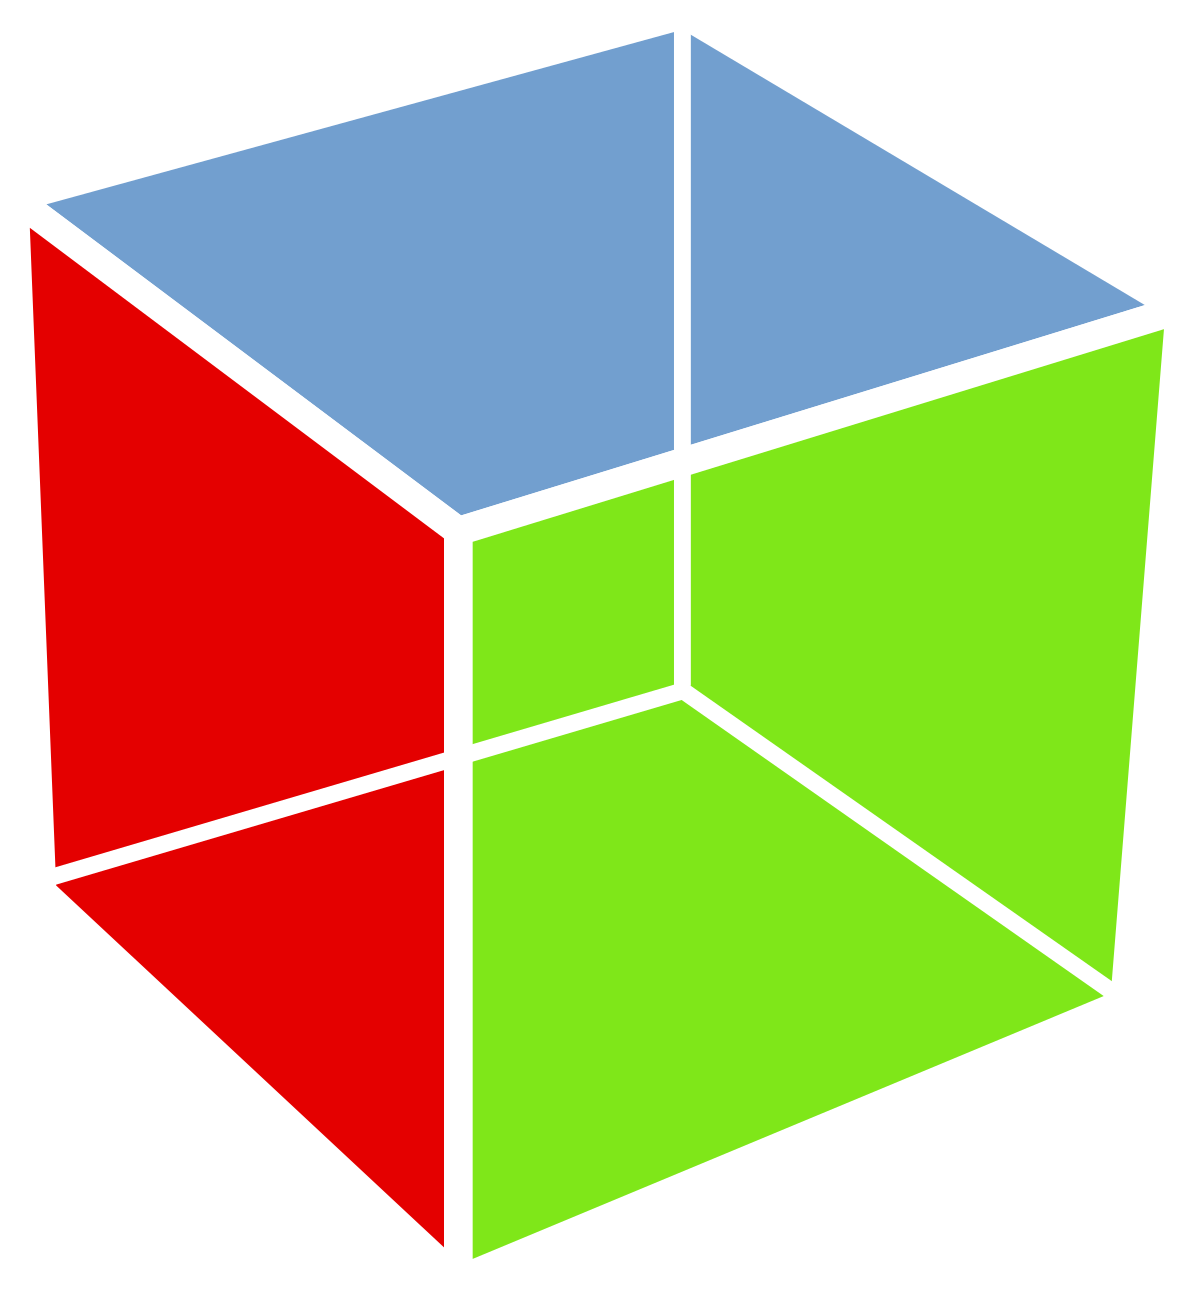
\includegraphics[width=0.4\textwidth]{GTK.PNG}
	  \caption{GTK}
	\label{fig:GTK}
\end{figure}
\section{Les interfaces graphiques}\label{sec:section2}
\subsection{Authentification}
	En premier lieu, l’utilisateur est censé d’accéder à son propre compte.
S’il est la première fois qu’il utilise l’application, l’utilisateur est censé de créer son propre compte.
\begin{figure}[H]
	\centering
	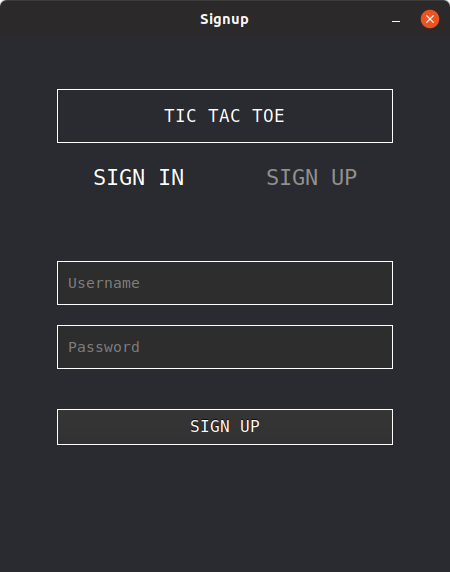
\includegraphics[width=0.4\textwidth]{sign up.PNG}
	  \caption{créer son propre compte}
	\label{fig:créer son propre compte}
\end{figure}
Sinon il va accéder directement à son compte, à travers l’interface d’authentification.
\begin{figure}[H]
	\centering
	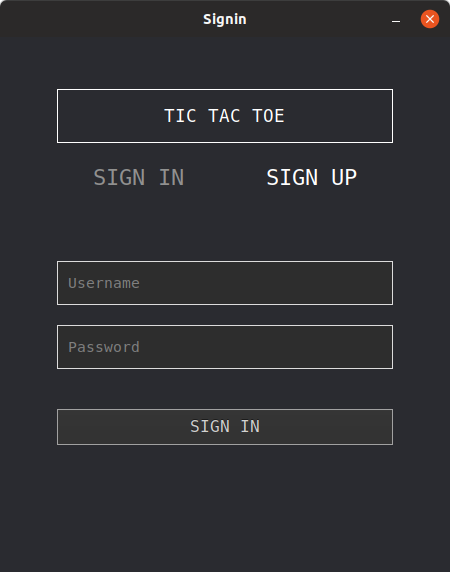
\includegraphics[width=0.4\textwidth]{sign in page .PNG}
	  \caption{page d'Authentification}
	\label{fig:page d'Authentification}
\end{figure}
\subsection{Accueil}
Après que le joueur accède à son compte, une interface d’accueil sera affichée en indiquant, les options disponibles :
\begin{figure}[H]
	\centering
	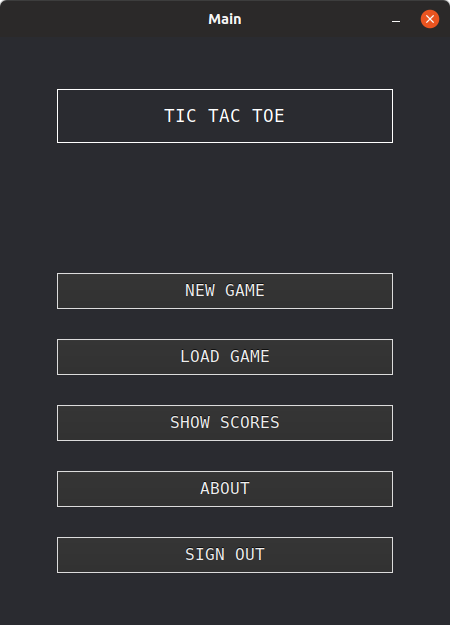
\includegraphics[width=0.4\textwidth]{main window.PNG}
	  \caption{La page pricipale}
	\label{fig:La page pricipale}
\end{figure}

\subsection{Nouvelle partie}
Si le joueur choisie de crée une nouvelle partie, il au choix entre jouer contre des mouvements aléatoires ou un algorithme (MiniMax Élagage alpha-bêta) .
\begin{figure}[H]
	\centering
	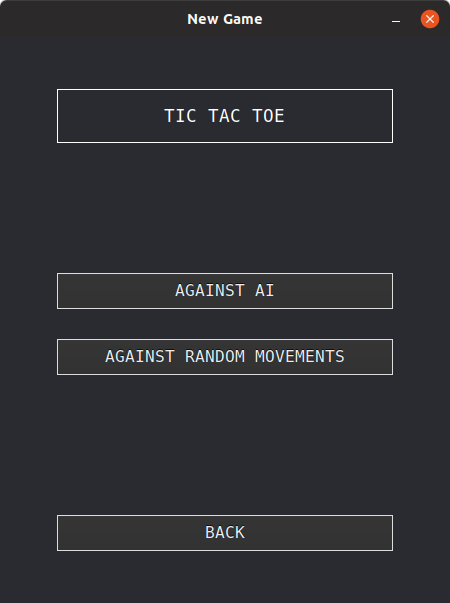
\includegraphics[width=0.4\textwidth]{new game button.PNG}
	  \caption{Nouvelle partie}
	\label{fig:Nouvelle Partie}
\end{figure}

Le signe du joueur (X) ou (O) est choisi arbitrairement,  à la fin de chaque partie un message montre le résultat : victoire, perte ou match nul 
\begin{figure}[H]
	\centering
	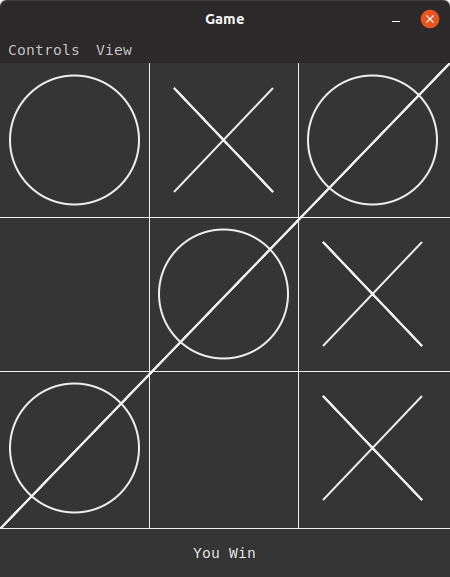
\includegraphics[width=0.4\textwidth]{win.PNG}
	  \caption{Le joueur gagne}
	\label{fig:Le joueur gagne}
\end{figure}
\begin{figure}[H]
	\centering
	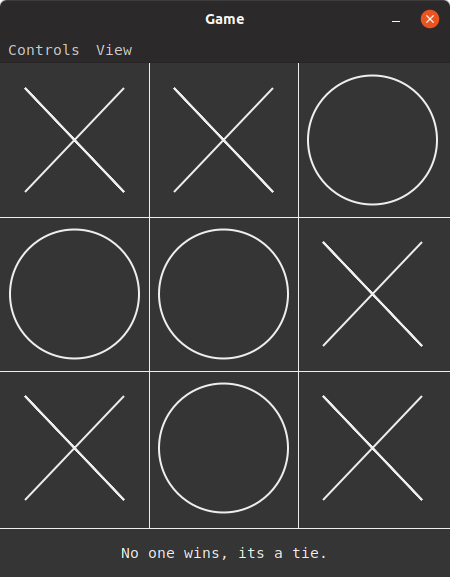
\includegraphics[width=0.4\textwidth]{tie .PNG}
	  \caption{Match nul}
	\label{fig:match nul}
\end{figure}
\begin{figure}[H]
	\centering
	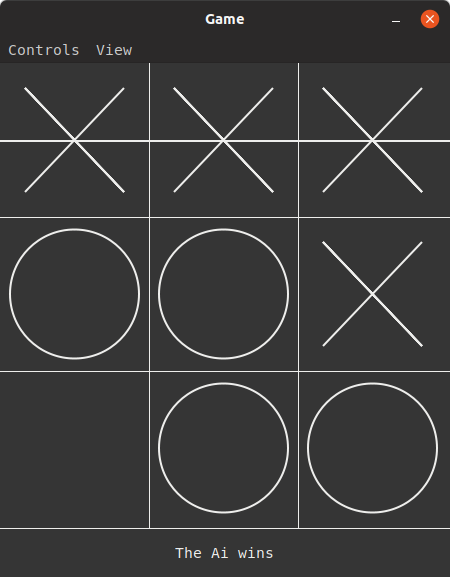
\includegraphics[width=0.4\textwidth]{loss against ai .PNG}
	  \caption{Le joueur perd}
	\label{fig:Le joueur perd}
\end{figure}
\clearpage
\subsubsection{Le menu de contrôle}
Aussi, durant la partie le joueur possède d’un menu de control, ce menu lui permet de Recommencer la partie, la Sauvegarder et pouvoir la continuer après ou quitter la partie et retourner vers le menu principal 
\begin{figure}[H]
	\centering
	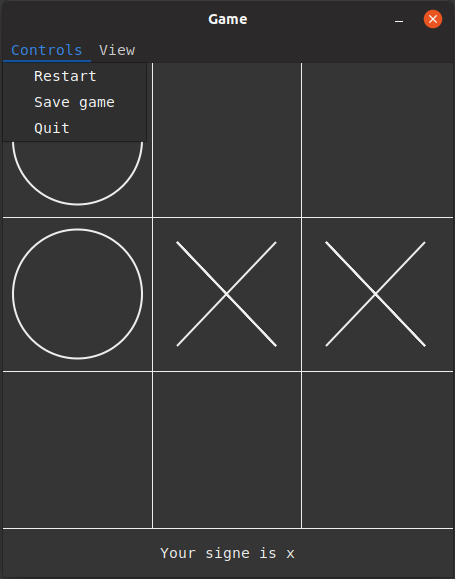
\includegraphics[width=0.4\textwidth]{control menu.PNG}
	  \caption{Le menu de contrôle}
	\label{fig:Le menu de contrôle}
\end{figure}
\subsubsection{L'historique}
Le menu (view) lui permet de voir l’historique des mouvements de chaque joueur 
\begin{figure}[H]
	\centering
	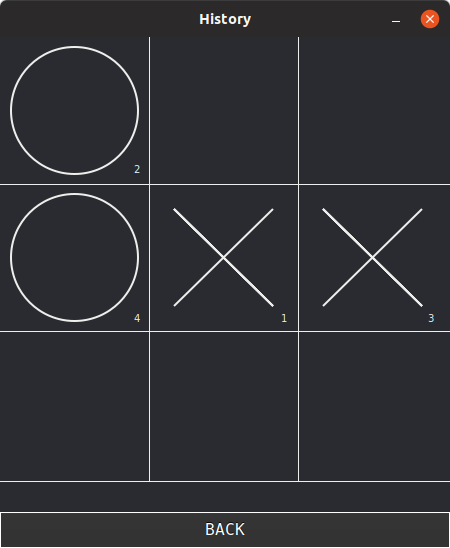
\includegraphics[width=0.4\textwidth]{history page.PNG}
	  \caption{L'historique}
	\label{fig:L'historique}
\end{figure}

\subsection{Charger une partie}
Le joueur est capable de continuer une partie déjà enregistrée par la sélectionner et cliquer sur le bouton (LOAD).
\begin{figure}[H]
	\centering
	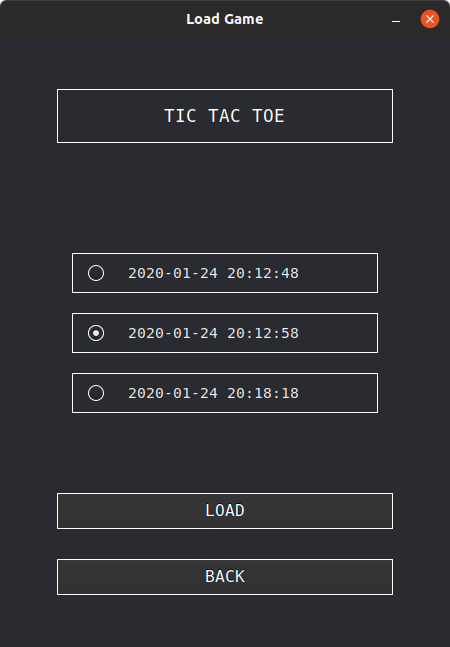
\includegraphics[width=0.4\textwidth]{select game to load.PNG}
	  \caption{Charger une partie}
	\label{fig:Charger une partie}
\end{figure}
\clearpage
\subsection{Afficher les scores}
A partir du menu principal, le joueur peut consulter les dix meilleurs scores de tous les joueurs :
\begin{figure}[H]
	\centering
	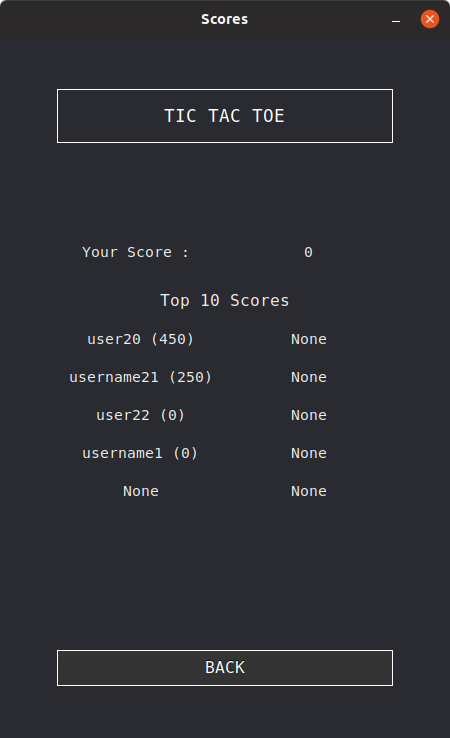
\includegraphics[width=0.4\textwidth]{scores page.PNG}
	  \caption{Afficher les scores}
	\label{fig:Afficher les scores}
\end{figure}
\clearpage
\subsection{A propos (about)}
Cette page contient le nom des contributeurs au projet 
\begin{figure}[H]
	\centering
	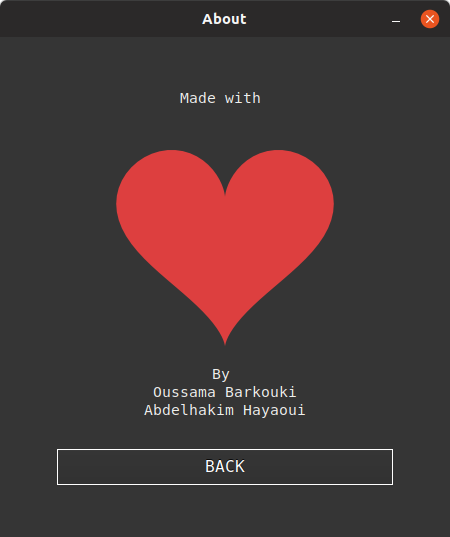
\includegraphics[width=0.4\textwidth]{about page .PNG}
	  \caption{A propos (about)}
	\label{fig:A propos (about)}
\end{figure}

 \textbf{\emph{A mentionner que le joueur peut toujours se déconnecter et retourner vers la page d’Authentification}}
\clearpage
\section{Les Limitations }\label{sec:section3}

\subsection{Nombre de parties enregistres }
Chaque joueur a le droit d’enregistrer jusqu’à  3 parties, au-delà il doit écraser la plus ancienne pour pouvoir enregistrer une nouvelle. 
\begin{figure}[H]
	\centering
	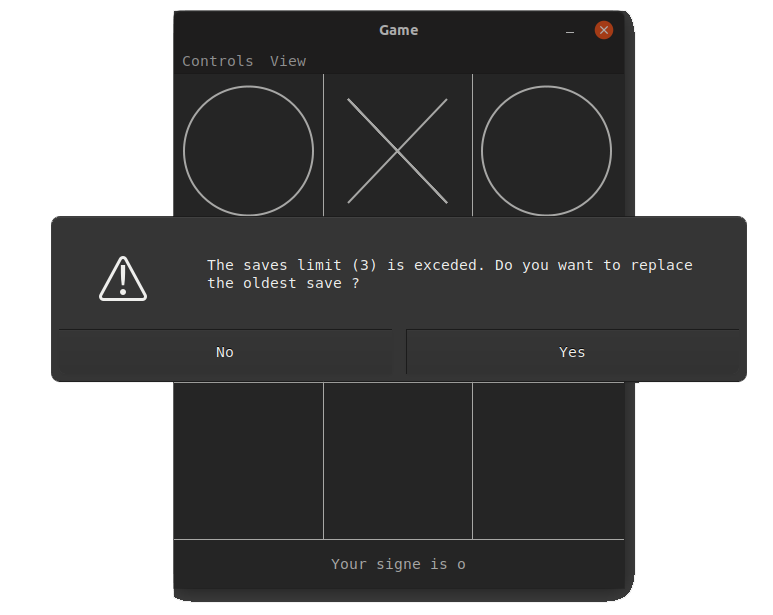
\includegraphics[width=0.4\textwidth]{exceded lmit saves finale.PNG}
	  \caption{Nombre de parties enregistres}
	\label{fig:Nombre de parties enregistres}
\end{figure}

\subsection{Une partie terminée }
Une partie terminée ne peut pas être enregistrée .

\begin{figure}[H]
	\centering
	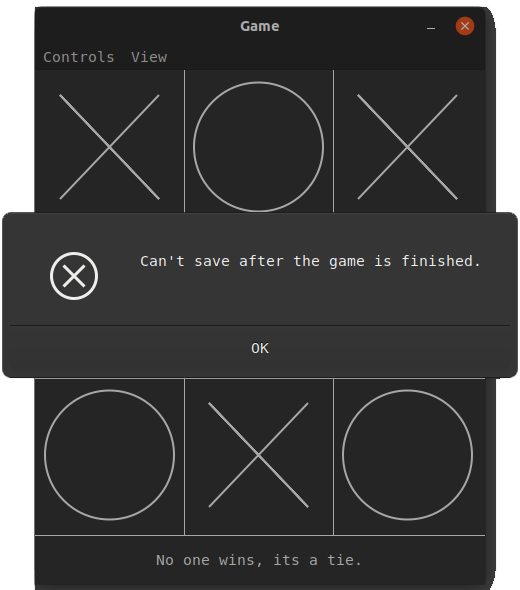
\includegraphics[width=0.4\textwidth]{cannot save if game ended.PNG}
	  \caption{Fin de la partie}
	\label{fig:Fin de la partie}
\end{figure}
\clearpage
\subsection{Utilisateur déjà existe  }
Si le nom d’utilisateur déjà existe un message va s’afficher

\begin{figure}[H]
	\centering
	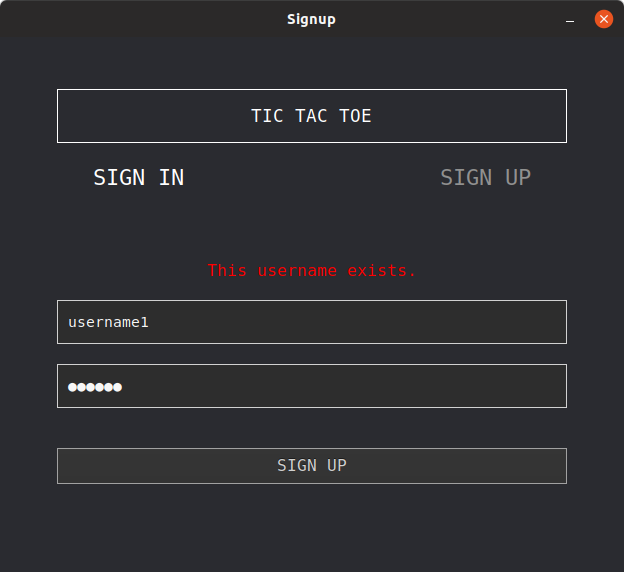
\includegraphics[width=0.4\textwidth]{user already exist.PNG}
	  \caption{Utilisateur déjà existe}
	\label{fig:Utilisateur déjà existe}
\end{figure}

\subsection{Spécifications du nom d’utilisateur }
Le nom d’utilisateur  ne peut pas être inférieur à 3 ou supérieur à 15 caractère.

\begin{figure}[H]
	\centering
	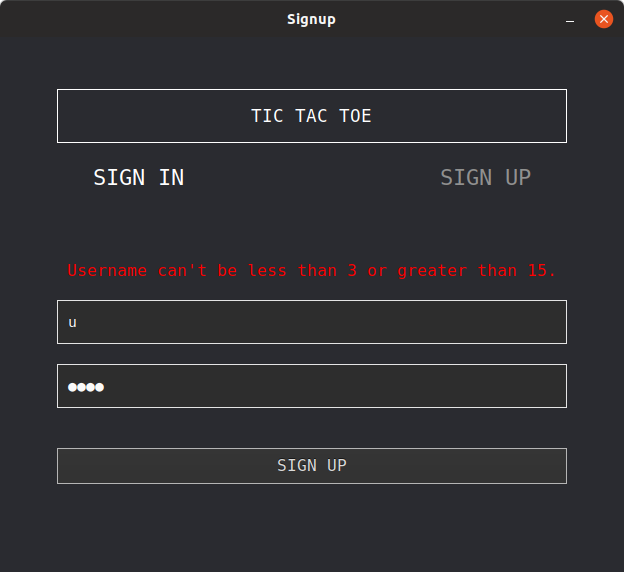
\includegraphics[width=0.4\textwidth]{username limitation.PNG}
	  \caption{Spécifications du nom d’utilisateur}
	\label{fig:Spécifications du nom d’utilisateur}
\end{figure}
\clearpage
\chapter{ Conclusion générale et perspectives  } \label{ch:structure}
Notre projet a consisté à la réalisation d’un jeu très populaire ‘’tic-tac-toe ‘’ 
Ce projet nous a permis d’approfondir nos connaissances théoriques, acquises tous le long de notre formation, par la pratique des nouvelles technologies. Cette expérience nous a permis de maîtriser le langage C ainsi que la bibliothèque utilisé qu’est GTK3+
Ce rapport explicite une première version du projet. L’ensemble des fonctionnalités demandées dans le cahier de charges ont été réalisées et implémentées dans le temps et fonctionnent correctement.
L’amélioration qu’on peut voir dans ce projet et le faite qu’il soit sous forme d’application mobile, puisque la base de ses utilisateurs est toujours en augmentation 

\chapter{ WEBOGRAPHIE} \label{ch:structure}
\url{https://github.com/oussama1598/tic_tac_toe} : lien du projet sur GitHub (sera publique après la soutenance)
% ############################################

% ############################################
% ############################################





% ----------------------------------------------


% ############################################


% ############################################


% ----------------------------------------------


% ############################################

% ############################################

	\clearpage

%%%%% Bibliography
	\fancyhead[LE,RO]{\nouppercase\leftmark}
	\printbibliography[heading=bibintoc]
	\cleardoublepage
%%%%% Appendix
	\fancyhead[LE,RO]{A  \ -- \ \nouppercase\leftmark}
	

\end{document}
